\documentclass{article}
 
\usepackage[T2A]{fontenc}
\usepackage[utf8]{inputenc}
\usepackage[bulgarian]{babel}
\usepackage{cite}
\usepackage{graphicx}
\usepackage{amsmath}
\usepackage{amsfonts}
\usepackage{float}
\usepackage{algpseudocode}
\usepackage{listings}
\usepackage{pgfplots}
\usepackage{amssymb}
\usepackage{xcolor}

\definecolor{codegreen}{rgb}{0,0.6,0}
\definecolor{codegray}{rgb}{0.5,0.5,0.5}
\definecolor{codepurple}{rgb}{0.58,0,0.82}
\definecolor{backcolour}{rgb}{0.95,0.95,0.92}

\lstdefinestyle{mystyle}{
	backgroundcolor=\color{backcolour},
	commentstyle=\color{codegreen},
	keywordstyle=\color{magenta},
	numberstyle=\tiny\color{codegray},
	stringstyle=\color{codepurple},
	basicstyle=\ttfamily\footnotesize,
	breakatwhitespace=false,
	breaklines=true,
	captionpos=b,
	keepspaces=true,
	numbers=left,
	numbersep=5pt,
	showspaces=false,
	showstringspaces=false,
	showtabs=false,
	tabsize=2
}

\lstset{style=mystyle}

\graphicspath{{images/}}

\title{Изследване на скалируемостта на Wa-Tor симулацията при cтатична декомпозиция на домейна}

\author{Иван-Асен Веселинов Чакъров \\
	ФН: 81837, Курс: 3, Група: 1}
\date{\today}


\begin{document}

\maketitle

\newpage

\tableofcontents

\newpage

\section{Увод}
Wa-Tor~\cite{wator} е класически проблем при паралелното програмиране.
Накратко проблемът е симулирането на идеализиран двумерен свят с формата на тор.
Светът има два вида обитатели - херинги, които играят ролята на плячка и акули, които ловят и изяждат херингите.
Подробните правилата за симулацията са дадени във~\cite{wator}.
\\
\\
Декомпозицията на домейн (Domain decomposition)~\cite{domain_decomposition}
при паралелното програмиране се явява естествен подход при решаването на проблеми,
при които за решаването на проблема за даден елемент $D$ от домейна са нужни само малко подмножество от данни,
които са "близо" до $D$. Накратко, идеята е, че разбиваме домейна на множество поддомейни
и възлагаме решаването на проблема за всеки поддомейн на отделен процес.
Важно е отделните поддомейни да са със еднаква големина за да може да се разпредели
хубаво работата между процесорите. Съществуват два вида Domain decomposition - статичен и динамичен.
При статичния в началото на алгоритъма разбиваме домейна и разпределяме работата между процесите.
По време на симулацията разбиването не се променя, което може да води до намаляване на производителността
тъй като данните при доста проблеми прескачат от един домейн в друг.
Този проблем се решава от втория тип Domain decomposition, който по време на симулацията
преизчислява разбиването на домейна с цел балансиране на големината на отделните поддомейни.
Domain decomposition намира приложение при решаването на проблеми от тип
Celular automata ~\cite{celular_automata}.
\\
\\
Тъй като и Wa-Tor попада в този тип проблеми, решението което представям тук е базирано
на статична декомпозиция на домейна.
\\
\\
разбивеме светът по редове (или по колони) на равни по големин ленти.

\section{Инструкции за употреба}
Програмата се разпространява по 2 основни начина:

\begin{itemize}
	\item Linux container (Docker): В този вид програмата носи със себе си всички неща на които зависи.
		За да се пусне на дадена машина трябва да има инсталиран Docker. Това е и използваният начин
		за изкарването на тестовите резултати.
	\item Java JAR: Стандартен начин за разпространие на Java базирани програми. Особеност е, че проектът
		е разработен на Java 16, като използва и експериментални функции на езика, така че
		препоръчаният начин за използване е през Linux container-a.
\end{itemize}

\bigbreak

Примерни команди в Bash за пускане на програмата:

\begin{lstlisting}[language=Bash, caption=Пускане на програмата през Docker]
docker run -e ARGS='
	$threads \
	$iterations \
	$sharks \
	$fish \
	$height \
	$width' \
	ivanasen-wator:0.0.1
\end{lstlisting}

\begin{lstlisting}[language=Bash, caption=Пускане на програмата директно през Java]
java -jar ivanasen-wator.jar \
	$threads \
	$iterations \
	$sharks \
	$fish \
	$height \
	$width
\end{lstlisting}

\bigbreak

Значение на аргументите:
\begin{itemize}
	\item \$threads: Брой нишки
	\item \$iterations: Брой итерации, през които да мине симулацията
	\item \$sharks: Брой акули
	\item \$fish: Брой херинги
	\item \$height: Височина на полето
	\item \$width: Широчина на полето
\end{itemize}

\bigbreak

Пример за резултатът от изпълнението, който се изкарва на стандартния изход:

\begin{lstlisting}[language=Bash]
NThreads: 1
Iterations: 100
Shark count: 10000
Fish count: 1000000
Height: 6000
Width: 3000
Execution time millis: 400143
\end{lstlisting}

Интересният ред е "Execution time millis", което е времето в милисекунди прекарано
изпълнявайки симулацията от началото на работата на първата $Worker$ нишка до края
на изпълнението на последната. Повече за $Worker$ нишките обясняваме във следващата секция.

\section{Описание на паралелния алгоритъм}
Алгоритъмът, който позлваме се базира на статична декомпозиция на домейна.
Начинът, по който работи е следният. Да кажем, че искаме да изпълним алгоритъма с N на брой нишки.
Разбиваме полето на $N$ на брой непрекъснати участъка (поддомейна) по редове като гледаме големината им
да е еднаква. Ако височината $H$ не се дели точно на $N$ прибавяме остатъка към последния поддомейн.
След това възлагаме всеки поддомейн на отделна нишка, която си изчислява симулацията само за него.
Друг подход за разбиване би бил по "правоъглници" , тоест да имаме по няколко поддомейна на ред.
Изборът да го направим по редове е по 2 причини. Едната е, че така всеки поддомейн си комуникира само
с 2 съседа вместо с 4, което намалява времето за комуникация между отделните нишки, а втората причина
е, че този алгоритъм е по-прост за реализация.
\\
\\
След като сме разпределили поддомейните на нишките начинът, по който те си синхронизират работата е следния.
Всяка нишка обработва своя участък по редове, като започва от най-горния. След като го обработи изпраща
съобщение, че е свършила работа по него на нишката, която отговаря за съседния горен участък.
След това обработва вътрешните си редове без да праща никакви съобщения на никого, подобно на еднонишкова
имплементация. Преди да стигне най-долния ред изчаква да получи съобщение от нишката отговаряща за съседния
долен участък, че си е свършила работа по нейния пръв ред. След като го е получила завършва с обработката
и на последния ред. Така завършва една итерация от Wa-Tor симулацията за една нишка. След това нишката
продължава със следващата итерация, пак започвайки от първия ред.

В нашата имплементация на този алгоритъм използваме нишки, семафори и споделена памет за комуникация.
Следва псевдокод на стъпките, които изпълнява една нишка за една итерация:

\newpage

Нека $rowMutex[i]$ е семафор с начална стойност 1 за $i \in 1...N$.
Този семафор играе ролята на мютекс за достъп до даден ред на полето с номер $i$.
Нека $isUpdated[i]$ е семафор с начална стойност 0 за $i \in 1...N$.
Отново тези семафори са номерирани по редовете на полето. Служат за уведомяване,
че първия ред от участъка на дадена нишка е обработен.
Нека $startRow$ и $endRow$ са съответно номера на първия и последния ред,
който дадена нишка трябва да обработи.
\bigbreak
\begin{algorithmic}
\For{$i\gets startRow; i \leq endRow; i\gets i + 1$}
	\State $nextRow\gets (i + 1) \% N$
	\If {$i = startRow$}
		\State \Call{Acquire}{$rowMutex[i]$}
	\ElsIf{$i = endRow$}
		\State \Call{Acquire}{$isUpdated[nextRow]$}
		\State \Call{Acquire}{$rowMutex[nextRow]$}
	\EndIf

	\State \Call{UpdateStateForRow}{$i$}

	\If {$i = startRow$}
		\State \Call{Release}{$rowMutex[i]$}
		\State \Call{Release}{$isUpdated[i]$}
	\ElsIf{$i = endRow$}
		\State \Call{Release}{$rowMutex[nextRow]$}
	\EndIf
\EndFor
\end{algorithmic}
\bigbreak
Както виждаме този псевдокод е малко по-формална версия на алгоритъма, който описахме с думи.

Друго интересно нещо при алгоритъма ни е начинът по който представяме двумерния свят, в който се намират
обитателите на Wa-Tor. Освен, че използваме двумерна матрица за представянето на клетките
имаме и масив от свързани списъци от класа Creature, който представлява обитателите на даден
ред от полето. Тоест ако искаме да обработим даден ред ние трябва да итерираме свързания списък.
Това спестява много посещения на празни клетки, които имплементацията само със двумерна матрица прави.

Цялостно, алгоритъма като имплементация е подобен на този във ~\cite{bounded_neighbours}, но е опростена
версия, тъй като използва статична декомпозиция на домейна, т.е. не правим никакъв Load balancing
по време на изпълнение и само разбиваме домейна в началото.

\newpage

\section{Архитектура}
Решението е имплементирано на Java 16 и използва вградените способности за паралелно програмиране
използвайки нишки и споделена памет:
\begin{itemize}
	\item Thread: Класът за нишка в Java
	\item ExecutorService: Упрявлява множество нишки в даден Thread pool
	\item ReentrantLock: Мютекс
	\item Semaphore: Семафор
\end{itemize}

Важно е да отбележим, че при имплементацията на JVM, която ползваме (OpenJDK 16) нишките са истински
на ниво операционна система, тъй като има стари версии на JVM и нови разработки като Project Loom,
при които се използва тъй наречения Green Thread модел, при който нишките се менежират от самата JVM
и позволяват мултиплексиране на много JVM нишки върху една ОС нишка.
\\
\\
Архитектурата на проекта използва статична декомпозиция на домейна и е направена по модела Master-Slaves,
тъй като имаме една главна нишка, която управлява множество Worker нишки, които извършват изчисленията
необходими за симулацията.
\\
\\
Ще отбележим по-важните класове на програмата:
\begin{itemize}
	\item Creature (и наследниците му Fish и Shark): В Creature е общата логика за това как се държи
		даден обитател в нашия свят. Fish и Shark съдържат специфичните правила, по които се движат
		по полето.
	\item State: Представлява имплементацията за състоянието, в което се намира нашия свят.
	\item Worker: Този клас имплементира Runnable. Той представлява кода, който се изпълнява от една нишка
		върху даден участък от света. Инстанциите на класа играят ролята на slaves в нашия модел.
	\item World: Този клас играе ролята на Master. В него се съдържа логиката за създаването и управлението на отделните
		Worker-и използвайки ExecutorService.
	\item Simulation: Създава World и мери времето за изпълнение на N на брой итерации на State.
	\item GuiSimulation: Създава World и показва в графичен вид в реално време как тече симулацията.
		Тук използваме Java Swing и AWT за целта.
\end{itemize}

На следващата страница представяме UML клас диаграма на проекта.

\begin{figure}[H]
	\centering
	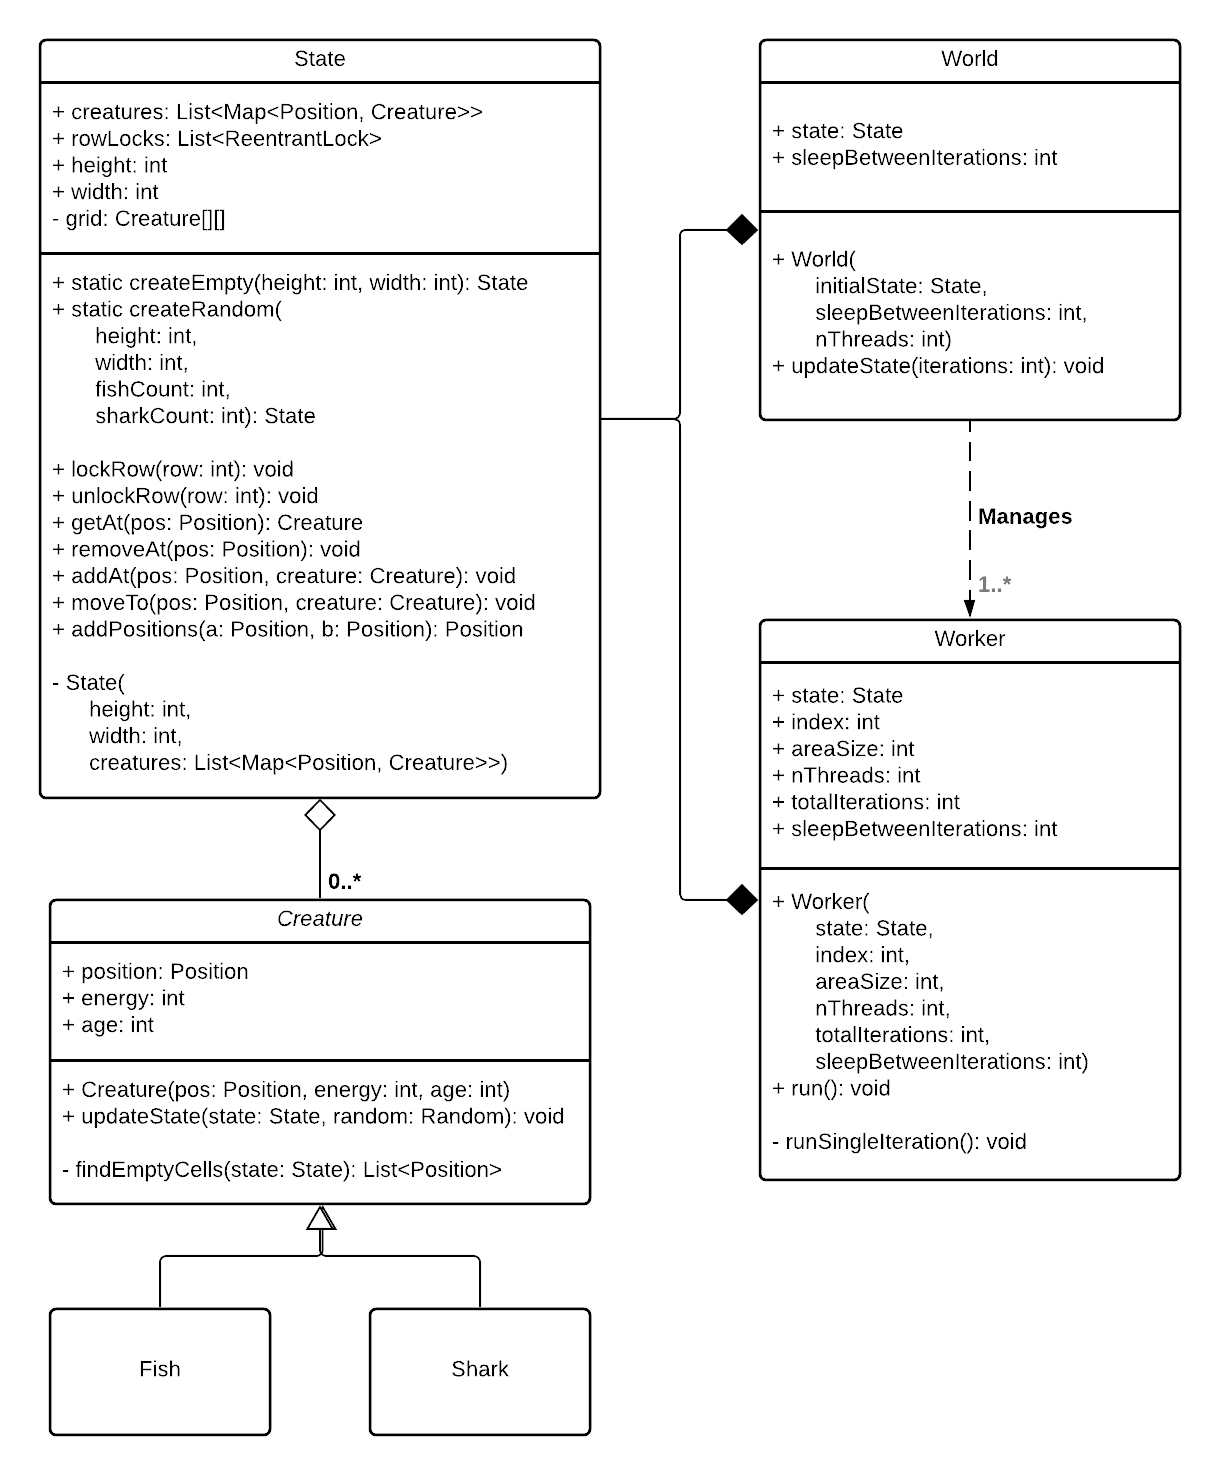
\includegraphics[width=1.2\textwidth]{classes-uml.png}
	\caption{UML Клас диаграма на проекта}
	\label{fig:figure1}
\end{figure}


\section{Тестови резултати}

Характеристики на тестовата машина: 
\begin{itemize}
	\item Процесор: 2 x Intel® Xeon® CPU E5-2660 0 @ 2.20GHz - Всеки процесор е с по 8 ядра и 2 нишки,
	това прави 16 ядра общо и 32 нишки (по 2 нишки на ядро благодарение на Hyperthreading).
	\item Памет: 64Gb, 32K L1d и L1i кешове, 256K L2 кеш и 20480К L3 кеш
\end{itemize}
Взимайки в предвид броя на нишките на машината има смисъл да тестваме скалируемост с до 32 паралелно работещи процеса/нишки.
\\
\\
Начинът по който са получени резултатите е следният. Пускаме симулацията да върви за $N$ итерации
и засичаме времето от началото на работата на всички нишки до края на работата на последната.
Правим отделни измервания от 1 до 32 нишки, като правим по 5 за всеки $K$ на брой нишки. След това
смятаме минимума, максимума и средното аритметично на получените резултати.
\\
\\
\begin{tabular}{ |p{0.6cm}||p{0.8cm}|p{0.8cm}|p{0.8cm}|p{0.8cm}|p{0.8cm}|p{0.8cm}|p{0.8cm}|p{0.8cm}|p{0.8cm}| }
 \hline
 \multicolumn{10}{|c|}{Тестове при размер на полето 2000x1000 и популация 50 000} \\
 \hline
 \# & p & $T^{(1)}_p$ & $T^{(2)}_p$ & $T^{(3)}_p$ & $T^{(4)}_p$ & $T^{(5)}_p$ & $T_p$ & $S_p$ & $E_p$ \\
 \hline
1  & 1  & 87521 & 85238 & 88839 & 88392 & 83791 & 83791 & 1.00 & 1.00 \\
2  & 2  & 43636 &  43001 & 42122 & 42790 & 42451 & 42122 & 1.98 & 0.99 \\
3  & 4  & 23608 & 23848 & 23023 & 21739 & 23980 & 21739 & 3.85 & 0.96 \\
4  & 8  & 15380 & 15380 & 17515 & 17541 & 22925 & 15380 & 5.44 & 0.68 \\
5  & 12 & 12934 & 10676 & 10307 & 9834 & 9906 & 9834 & 8.52 & 0.71 \\
6  & 16 & 9089 & 9315 & 9004 & 9134 & 9245 & 9004 & 9.31 & 0.58 \\
7  & 20 & 8826 & 9019 & 8913 & 9056 & 9033 & 8826 & 9.49 & 0.47 \\
8  & 24 & 8716 & 8628 & 9207 & 9010 & 8833 & 8628 & 9.71 & 0.40 \\
9  & 28 & 9462 & 9054 & 9910 & 9264 & 9493 & 9054 & 9.25 & 0.33 \\
10 & 32 & 10150 & 9903 & 10275 & 10361 & 9935 & 9903 & 8.46 & 0.26 \\
 \hline
\end{tabular}
\\
\\
\\
\begin{tabular}{ |p{0.6cm}||p{0.8cm}|p{0.8cm}|p{0.8cm}|p{0.8cm}|p{0.8cm}|p{0.8cm}|p{0.8cm}|p{0.8cm}|p{0.8cm}| }
 \hline
 \multicolumn{10}{|c|}{Тестове при размер на полето 4000x2000 и популация 1 000 000} \\
 \hline
 \# & p & $T^{(1)}_p$ & $T^{(2)}_p$ & $T^{(3)}_p$ & $T^{(4)}_p$ & $T^{(5)}_p$ & $T_p$ & $S_p$ & $E_p$ \\
 \hline
1  & 1  & 1.00  & 1.00 & 1 & 1 & 1 & 1 & 1 & 1 \\
2  & 2  & 1.00  & 1.00 & 1 & 1 & 1 & 1 & 1 & 1 \\
3  & 4  & 1.00  & 1.00 & 1 & 1 & 1 & 1 & 1 & 1 \\
4  & 8  & 1.00  & 1.00 & 1 & 1 & 1 & 1 & 1 & 1 \\
5  & 12 & 1.00  & 1.00 & 1 & 1 & 1 & 1 & 1 & 1 \\
6  & 16 & 1.00  & 1.00 & 1 & 1 & 1 & 1 & 1 & 1 \\
7  & 20 & 1.00  & 1.00 & 1 & 1 & 1 & 1 & 1 & 1 \\
8  & 24 & 1.00  & 1.00 & 1 & 1 & 1 & 1 & 1 & 1 \\
9  & 28 & 1.00  & 1.00 & 1 & 1 & 1 & 1 & 1 & 1 \\
10 & 32 & 1.00  & 1.00 & 1 & 1 & 1 & 1 & 1 & 1 \\
 \hline
\end{tabular}
\\
\begin{tikzpicture}
\begin{axis}[
	title={Време за изпълнение при размер на полето 4000x2000},
	xlabel={Брой нишки},
	ylabel={Време в секунди},
	legend pos=north west,
	ymajorgrids=true,
	grid style=dashed,
]
\\
\addplot[
	color=blue,
	mark=square,
	]
	coordinates {
	(1,517)(6,105)(11,70)(16,59)(21,54)(26,51)(31,50)
	};

\end{axis}
\end{tikzpicture}

\begin{tikzpicture}
\begin{axis}[
	title={Средно ускорение при размер на полето 4000x2000},
	xlabel={Брой нишки},
	ylabel={Ускорение},
	legend pos=north west,
	ymajorgrids=true,
	grid style=dashed,
]

\addplot[
	color=blue,
	mark=square,
	]
	coordinates {
	(1,1)(6,4.9)(11,7.4)(16,8.6)(21,9.4)(26,10)(31,10.3)
	};
\addlegendentry{Реално ускорение}

\addplot[
	domain=0:31,
	color=green
]{0.7 * x};
\addlegendentry{Идеално ускорение}
\end{axis}
\end{tikzpicture}

\begin{tikzpicture}
\begin{axis}[
	title={Средно ускорение при размер на полето 4000x2000},
	xlabel={Брой нишки},
	ylabel={Ускорение},
	legend pos=north west,
	ymajorgrids=true,
	grid style=dashed,
]

\addplot[
	color=blue,
	mark=square,
	]
	coordinates {
	(1,1)(6,4.9)(11,7.4)(16,8.6)(21,9.4)(26,10)(31,10.3)
	};
\addlegendentry{Реално ускорение}

\addplot[
	domain=0:31,
	color=green
]{0.7 * x};
\addlegendentry{Идеално ускорение}
\end{axis}
\end{tikzpicture}


\section{Визуализации}
Освен симулацията, която служи за измервание на скалируемостта,
в проекта е разработена и визуализация в реално време с помощта на Java Swing и AWT.
Следват няколко екранни снимки от визуализации (херингите са в зелено, а акулите в синьо):

\begin{figure}[H]
	\centering
	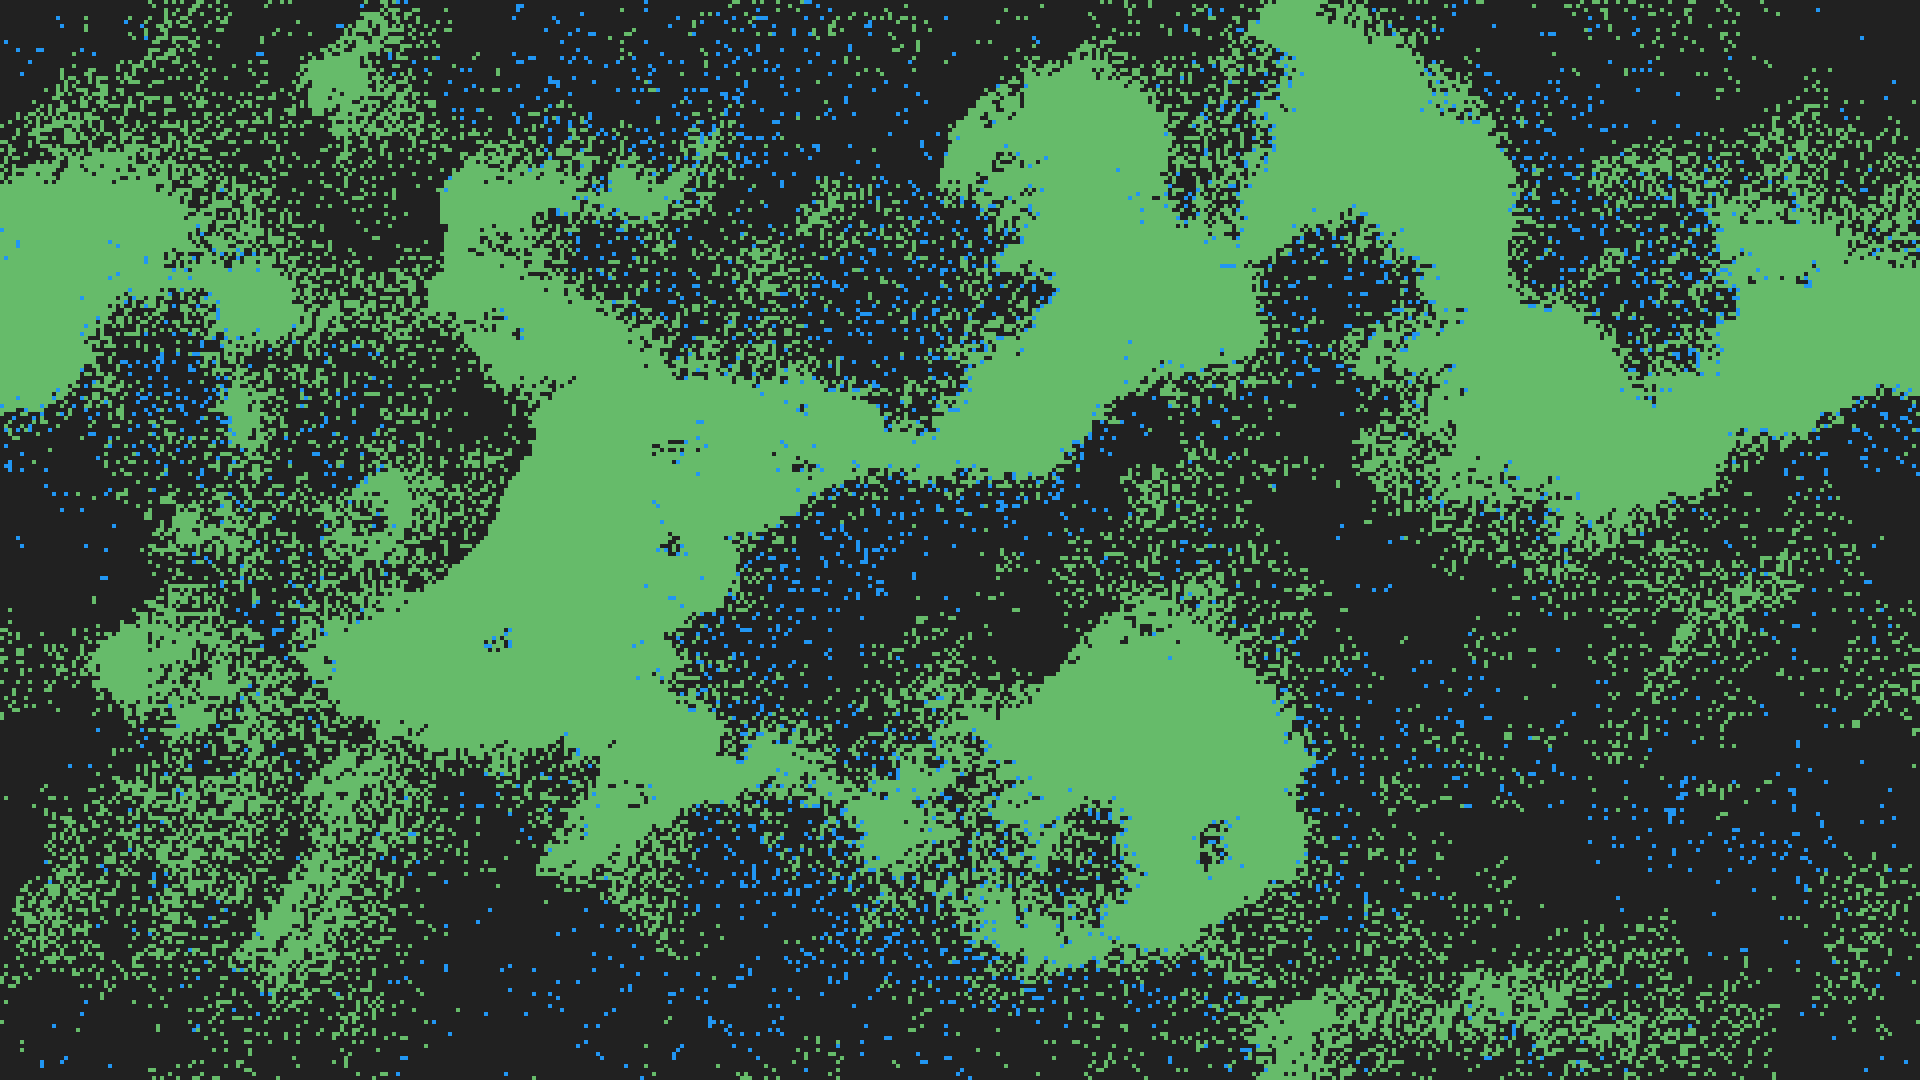
\includegraphics[width=1\textwidth]{screenshot-small.png}
	\caption{Размер на полето 480x270, 10 000 херинги и 1000 хиляди акули}
\end{figure}

\begin{figure}[H]
	\centering
	
\includegraphics[width=1\textwidth]{screenshot-big.png}
	\caption{Размер на полето 1920x1080, 1 000 000 херинги и 100 000 акули}
\end{figure}

Първоначалната цел на този "режим на работа" беше лесен начин за дебъгване,
но в крайна сметка се получи и доста готина анимация, която би могла да се ползва за screensaver :).

\section{Бъдещо развитие на проекта}
Резултатите, които са получени при статична декомпозиция на домейна са сравнително хубави,
но е възможно да се подобрят с използването на динамична декомпозиция, тоест да правим
load balancing на отделните домейни по време на изчисленията. Това помага особено при
по-голям размер на полето. Примерни резултати за това какво може да бъде постигнато при
използването на такъв тип алгоритъм са дадени във ~\cite{bounded_neighbours} използвайки
алгоритъм наречен "Bounded neighbours".
\bibliography{wator}{}
\bibliographystyle{plain}
\end{document}
